\chapter{Termokamera}
Pro pochopení řešení této práce je nutné se seznámit s~technologií termokamer a dalšími důležitými pojmy  z~termografického oboru. Technologie a způsob použití je proti běžným kamerám rozdílná a má tedy smysl se jejím popisem zabývat.

Oblast termografie je sama o~sobě velmi náročná a mohla by být samostatným tématem rozsáhlé vědecké práce. Kapitola se věnuje pouze základním principům a pro detailnější pochopení této oblasti jsou doporučeny práce \cite{kaplan2007practical,gaussorgues2012infrared,vollmer2010infrared}.

\section{Co je to termokamera}
Termokamera je zařízení, které nám umožňuje zobrazit a zaznamenat námi jinak neviditelné infračervené záření. Podobným způsobem jako běžné kamery zaznamenávají viditelné spektrum. 

\begin{figure}[h]
  \centering
  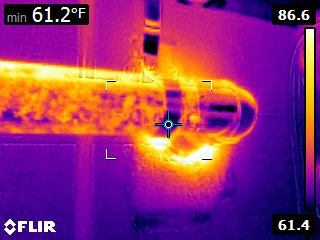
\includegraphics[width=0.7\textwidth]{images/thermal_camera_sample_image.jpg}
  \caption{Ukázkový snímek pořízený termokamerou \cite{thermalSampleImage}}
\end{figure}

\section{Princip snímání} \label{section:measurement_principle}
Snímání termokamery spočívá v~bezdotykovém měření povrchové teploty těles. Tento způsob využívá skutečnosti, že každé těleso, jehož teplota je vyšší než absolutní nula, vyzařuje tepelné záření \cite{puhl2015bezkontaktni, kadleckzadkladymereni1}. Jak se těleso stává teplejším, ve vnitřní struktuře se zrychluje pohyb atomů a molekul, a tím se tvoří více energie, kterou je potřeba vyzářit. Snímač termokamery (detektor) infračervené spektrum zaznamenává formou elektronických signálů, který jsou následně digitalizovány a převedeny na termografický snímek. 

Technologicky není možné konstruovat snímače termokamery tak, aby zachytily celý rozsah infračerveného spektra. Proto jsou vždy konstruovány pro konkrétní infračervenou oblast. V~dnešní době je to nejčastěji oblast LWIR (více o~oblastech v~\ref{sec:ir_radiation}) a to díky nižší ceně technologie a velmi dobrým výsledkům.    
    
   	\subsection{Absolutní nula}
    Absolutní nula je teoretický stav tělesa, při kterém se zastaví veškerý pohyb částic a z~tělesa již nelze odebírat žádné další teplo. Hodnota absolutní nuly je 0~kelvinů neboli -273,15 \textdegree{}C. Zatím neexistuje známý způsob, jak 0 K~dosáhnout. Jsou pouze známy způsoby a byly provedeny experimenty, které se k~dosáhnutí hodnoty absolutní nuly limitně přibližují. 
       
    \subsection{Elektromagnetické záření}
       Elektromagnetické záření je příčné postupné vlnění tvořené elektrickým a magnetickým polem. Lidé nejčastěji vnímají záření nazývané viditelné spektrum neboli světlo, které nám umožňuje vidět. Kromě viditelného spektra bylo postupem času objevováno více druhů záření, které bylo nutné rozdělit do skupin. Tyto skupiny tvoří takzvané elektromagnetické spektrum, kde jsou jednotlivá záření popsána jejich vlnovými délkami (respektive frekvencemi). Přechody mezi skupinami jsou plynulé a některé se částečně překrývají. 
       
       Záření, které lidskému oku umožňuje vidět se nazývá viditelné spektrum. Viditelné spektrum lze nalézt  mezi UV a IR zářením, a to pouze ve velmi úzkém rozsahu vlnových délek od 400 nm do 800 nm. Záření mimo viditelné spektrum je pro lidstvo nejen neviditelné, ale lidé jej nedokáží ani vnímat. Přesto je možné se zářením různých druhů dennodenně setkávat. Příkladem je ultrafialové záření, jehož zdrojem je slunce a lidský organismus ovlivňuje tvorbou kožních skvrn a přispívá na tvorbě vitamínu D. Na rozdíl od lidí však existují živočichové, kteří jsou schopni vnímat nejen viditelné spektrum, ale také UV a IR spektrum. \cite{smrvz2013bezkontaktni, kadleckzadkladymereni1} 
                   
    \begin{figure}[h]
      \centering
      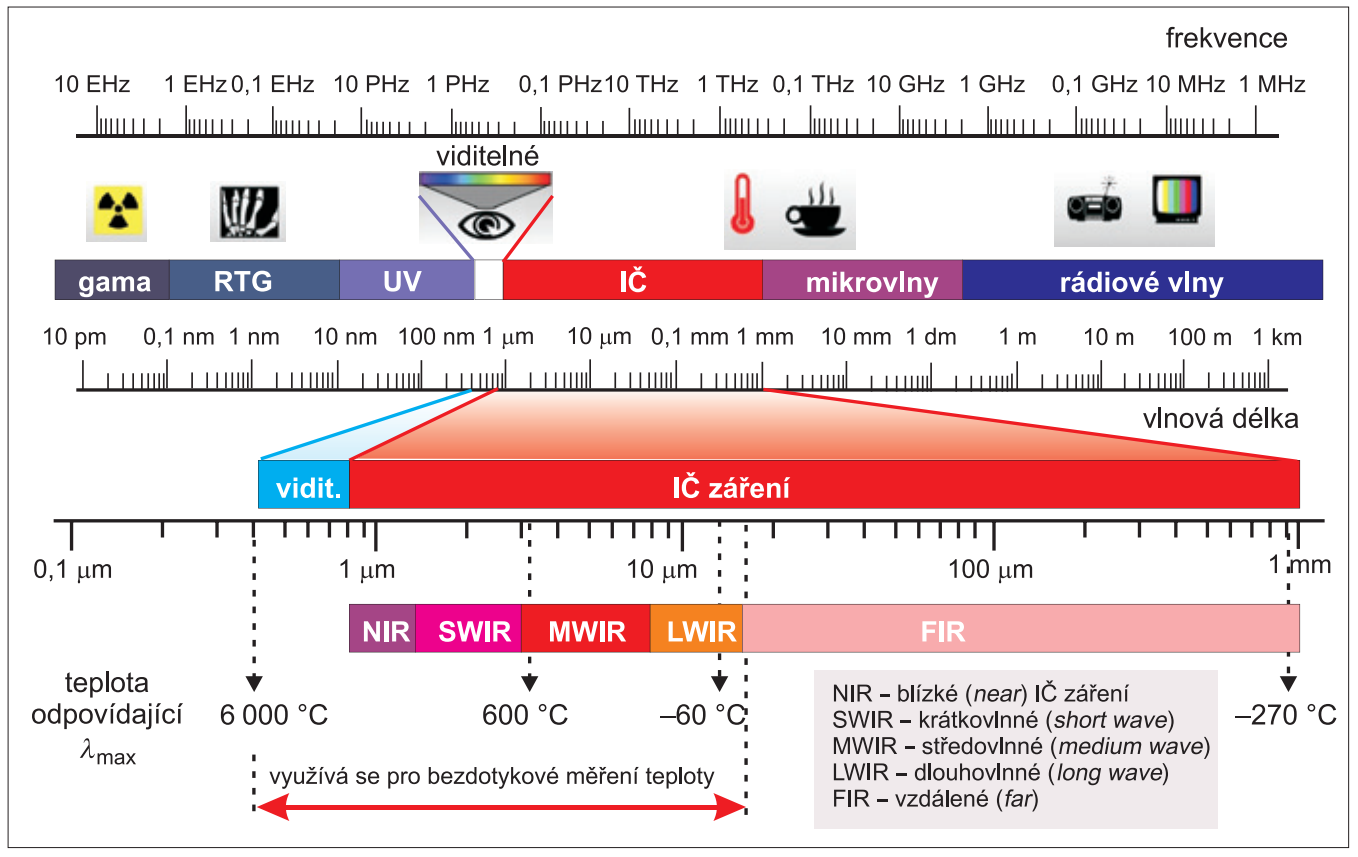
\includegraphics[width=1\textwidth]{images/elektromagneticke_spektrum.png}
      \caption{Elektromagnetické spektrum s~vyznačenými pásmy infračerveného záření 								\cite{kadleckzadkladymereni1}}
    \end{figure}
    
    \subsection{Infračervené záření} \label{sec:ir_radiation}
    Infračervené záření je pouze jedna ze skupin patřící do celku elektromagnetických záření. Jeho vlnová délka je přibližně od 760 nm do 1 mm a nachází se mezi viditelným spektrem a mikrovlnami.  \cite{stupvnankova2009ir} 
        
        Vlnová délka IR záření je závislá na teplotě tělesa, které jej vyzařuje. Obecně platí, že čím je teplota tělesa vyšší, tím se vlnová délka zkracuje \cite{kadleckzadkladymereni1}. IR záření se dále dělí na jednotlivá pásma, která však nejsou striktně daná a existuje více využívaných rozdělení \cite{stupvnankova2009ir}. Nejčastěji se však využívá obecné rozdělení uvedené v~tabulce \ref{table:ir_regions_table_common}. V~jiných zdrojích se též vyskytuje:

    \begin{itemize}[noitemsep]
      \item rozdělení dle doporučení od Mezinárodní organizace pro osvětlování (CIE),
      \item rozdělení dle normy ISO 20473,
      \item astronomické rozdělení.
    \end{itemize}

    \begin{table}[h]
      \centering
      \begin{tabular}{|c|c|c|c|}
        \hline
        \rowcolor{Blue}
        \color{White}\textbf{Název pásma} & \color{White}\textbf{Zkratka} & \color{White}\textbf{Rozsah od} & \color{White}\textbf{Rozsah do} \\ \hline
        blízké infračervené záření 	& NIR  		& 0.76 µm   & 1.4 µm   	    \\ \hline
        krátké vlnové délky   		& SWIR		& 1.4 µm 	& 3 µm		    \\ \hline
        střední vlnové délky 		& MWIR 		& 3	µm 		& 8 µm		    \\ \hline
        dlouhé vlnové délky  		& LWIR 		& 8 µm		& 15 µm		    \\ \hline
        vzdálené infračervené záření & FIR  	& 15 µm		& 1000 µm 	    \\ \hline
      \end{tabular}
      \caption{Obecné rozdělení oblastí infračerveného záření}
      \label{table:ir_regions_table_common}
    \end{table}
     
     \subsection{Absolutně černé těleso} \label{sec:absolute_black_body}
   	 Absolutní černé těleso  je ideální teoretické těleso, které pohlcuje veškeré dopadající záření všech vlnových délek. Současně s~touto vlastností se chová jako ideální zářič. To znamená, že ze všech možných těles o~stejné teplotě vyzařuje nejvíce energie. 
     
     V~reálném světě se absolutně černému tělesu blíží některé hvězdy a nebo vyrobené přístroje, pomocí kterých  jsou termokamery kalibrovány. \cite{kadleckzadkladymereni1, jakl2011experimentalni}
    
    Černé těleso si lze představit jako dutinu s~matným černým povrchem a~malým vstupním otvorem stejně jako je ilustrováno na obrázku \ref{fig:black_body_image}. Jakmile záření projde otvorem do trubky, po několika odrazech se úplně pohltí. Tedy veškeré záření, které se do absolutně černého tělesa dostane, se již zpět ven neodrazí. Pohlcené vstupní záření se přemění na energii a je zpět vysíláno pouze ve formě tepelného záření.
   
    \begin{figure}[h]
      \centering
      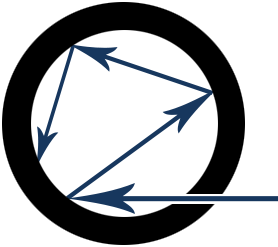
\includegraphics[width=0.3\textwidth]{images/black_body.png}
      \caption{Konceptuální černé těleso}
      \label{fig:black_body_image}
    \end{figure}    
     
\section{Konstrukce}
Všechny termokamery se skládají z~minimálně třech důležitých součástí, kterými jsou: optická soustava, detektor a obvody pro předzpracování obrazu \cite{jakl2011experimentalni,smrvz2013bezkontaktni,malik2012zpracovani}. Jednoduché schéma termokamery je možné vidět na obrázku \ref{fig:thermal_camera_scheme}. 

Základní a nejednoduší dělení termokamer je podle přítomnosti ovládacích prvků \cite{kuvzel2010bezkontaktni}. Toto dělení probíhá na:

\begin{description}[align=left]
  \item [Stacionární termokamery] obvykle využívané v~průmyslu, v~bezpečnosti, pro monitoring, apod. Stacionární kamery jsou  trvale připojeny k~počítači, který řídí jejich nastavení a přenos snímků. Obsahují pouze konektor pro připojení a nemají žádné ovládací prvky a většinou ani úložiště a baterii.
  \item [Ruční termokamery] jsou přenosné a nezávislé na počítači. Využívají se zejména pro snímkování v~terénu. Na rozdíl od stacionárních kamer obsahují vestavěnou baterii, ovládací prvky a LCD displej.
\end{description}
    
\begin{figure}[h]
  \centering
  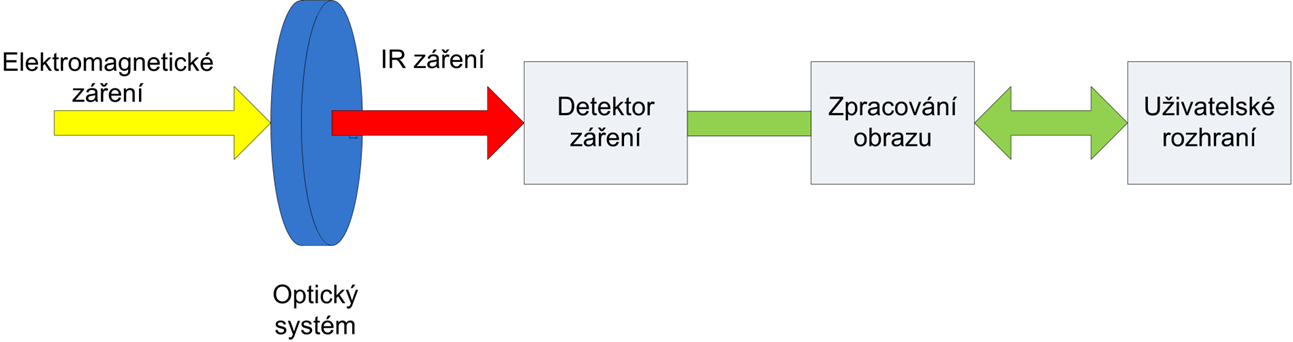
\includegraphics[width=1\textwidth]{images/konstrukce_kamery.png}
  \caption{Jednoduché schéma součástí termokamery \cite{konstrukcetermokamery}}
  \label{fig:thermal_camera_scheme}
\end{figure}
    
    \subsection{Detektor}
    Detektor  plní podobnou činnost jako snímač u~běžných RGB kamer. Na~detektor je pomocí optiky soustředěno infračervené záření, které je převáděno na elektronický signál. Signál je následně předzpracovaný korekcemi v~dalších přídavných obvodech a pak teprve převeden na výsledný snímek. Obvody pro předzpracování signálu jsou již nejčastěji součástí detektoru. \cite{smrvz2013bezkontaktni}
    
    Samotné signály z~detektoru bez aplikovaných korekcí lze zobrazit, ale výsledný obraz je velmi nekvalitní a navíc s~velkým počtem nepřesností. Pro představu je přiložen obrázek \ref{fig:flir_signal_image}, kde firma FLIR v~roce 2012 prezentovala výsledky svých nových algoritmů pro zpracování signálu z~detektoru.  Z~obrázku je patrné, že obvody pro zpracování signálu jsou velmi důležitou součástí termokamer.
    
    \begin{figure}[h]
      \centering
      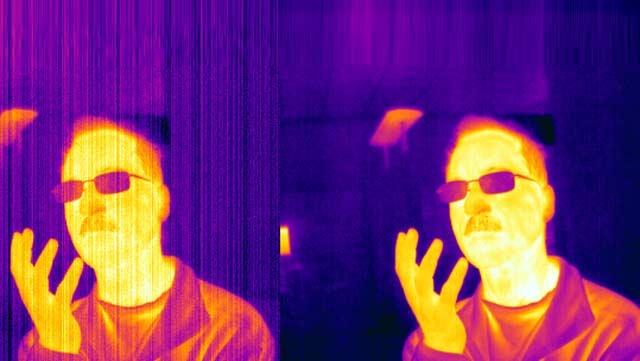
\includegraphics[width=0.6\textwidth]{images/flir_filter_with_without.jpg}
      \caption{Vlevo je snímek bez aplikovaných korekcí signálu a vpravo je snímek po aplikaci vhodných algoritmů zpracování signálu v~příslušných obvodech \cite{flirFPGAsignal}}
      \label{fig:flir_signal_image}
	\end{figure}    
    
    Termokamery lze dělit i podle druhu detektoru. Tyto dvě skupiny jsou výsledkem konstrukční technologie a jedná se o~dělení na chlazené a nechlazené detektory.
        
	\begin{description}[align=left]\label{description:detector_types}
      \item [Chlazené detektory,] někdy též označovány jako kvantové, přináší velmi přesné měření teplot, vysokorychlostní snímání, řádkové snímání (až 62~000 FPS v~případě \cite{flirSc7000}) a lepší zpracování šumu. V~závislosti na materiálu detektoru lze přizpůsobit pro IR oblasti SWIR, MWIR a LWIR. Kvůli nutnému chlazení mají větší rozměry a jejich váha se pohybuje v~jednotkách kg. Nevýhodou je několikanásobně vyšší cena oproti nechlazeným detektorům.
      \item [Nechlazené detektory] jsou konstrukčně jednodušší, spolehlivější, mají menší energetickou spotřebu a jsou cenově dostupné veřejnosti. V~dnešní době jsou nejčastější nechlazené detektory na bázi mikrobolometrů. Zajímavostí je fakt, že se dá dosáhnout velmi kompaktních rozměrů. Například detektory FLIR řady Lepton mají rozměry přibližně 1 $\times$ 1 $\times$ 0.7 cm. Tyto detektory se pouze ojediněle objevují pro jinou IR oblast než je LWIR. Nevýhody nechlazených detektorů jsou méně kvalitní výstup a~menší přesnost měření oproti chlazeným detektorům.
    \end{description}
        
    Chlazené detektory jsou velmi specifickou záležitostí, týkající se převážně extrémních využití (záchranné a bezpečnostní složky, armáda, vědecké a výzkumné ústavy, apod.), jejich popis a bližší informace nebudou součástí této práce. Podrobné detaily o~těchto detektorech lze nalézt v~knihách \cite{daniels2010field, rogalski2010infrared}.
        
    Naopak s~nechlazenými detektory je možné se setkat téměř ve všech běžných případech. Technologie nechlazených detektorů využívá výhradně mikrobolometrického pole \cite{vojavcekco, jakl2011experimentalni}. Toto dvourozměrné pole je složeno z~miniaturních bolometrů, které jsou citlivé na dopadající infračervené záření. Jednotlivé bolometry mění své elektrické odpory v~závislosti na množství tepelného záření snímaného tělesa. Každý odpor znamená jednu hodnotu signálu a jeden výsledný pixel obrazu. Rozlišení nechlazených detektorů je dáno počtem uspořádaných bolometrů v~matici. 
    
    \begin{figure}[h]
      \centering
      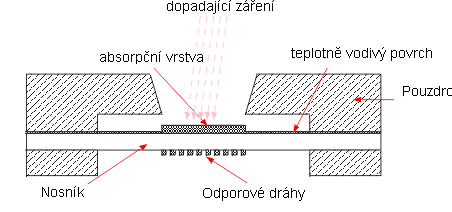
\includegraphics[width=0.6\textwidth]{images/bolometer_scheme.png}
      \caption{Schéma bolometru \cite{vojavcekco}}
      \label{fig:bolometer_scheme}
	\end{figure}  
    
    Rozlišení termokamer se obecně v~porovnání s~RGB kamerami pohybuje na skromnějších hodnotách. Od dnešních nejnižších rozlišení 80 $\times$ 60 pixelů až po extrémní třídu s~1024 $\times$ 1024 pixely. Je to z~toho důvodu, že pro dosažení dvojnásobného rozlišení termokamery,  je nutné čtyřnásobné zvětšení počtu bolometrů v~matici.
    
	\subsection{Optická soustava}
     Termokamery nemohou využívat běžnou optiku ze skla, tak jako ji využívají klasické kamery. Je to z~toho důvodu, že běžná optika infračervené záření převážně odráží než propouští. V~dnešní době již existuje více druhů používaných materiálů pro objektivy termokamer, ale nejčastěji se využívá germánium nebo jeho slitina.  \cite{kadlecsovatermokamery,stupvnankova2009ir}
     
     Optika z~germánia slouží také jako filtr všech ostatních vlnových délek a~k~samotnému detektoru, v~případě germánia, se dostává pouze záření z~pásma LWIR nebo MWIR (v~závislosti na úpravách optiky). Na optice jsou dále naneseny antireflexní nano vrstvy pro zvýšení propustnosti infračerveného záření. Optika a nano vrstvy termokamer jsou velmi šetrné a neodborným zacházením mohou být způsobena nevratná poškození. 
     
     Optika bohužel přichází o~své vlastnosti i postupem času. Jedná se zejména o~vnější vlivy, které způsobují její oxidaci a tím snižují propustnost infračerveného záření. Více o~volbách optických materiálů a jejich porovnání lze nalézt v~článku \cite{vandervlugtchoosing}.
     
\section{Specifikace a parametry}\label{sec:thermal_camera_features}
Seznam důležitých parametrů ovlivňující klíčovou funkčnost a možnosti termokamer jsou uvedeny v~tabulce \ref{table:thermal_camera_features}. K~jednotlivým parametrům je vždy uveden příklad a vysvětlující komentář.
    
\begin{table}[h]
	\centering
    \begin{tabular}{|p{4.5cm}|p{3cm}|p{6cm}|}
      \hline
      \rowcolor{Blue}
      \color{White}\textbf{Parametr} & \color{White}\textbf{Příklady} & \color{White}\textbf{Komentář}   \\ \hline
      Rozlišení detektoru & 240 $\times$ 180 pixelů &  Obecně platí, že vyšší je lepší. \\  \hline
      Typ detektoru & nechlazený FPA & Chlazený (kvantový) nebo nechlazený, více v~\ref{description:detector_types}.\\  \hline
      Snímané spektrum & LWIR, MWIR & Snímaná část IR spektra, více v~\ref{sec:ir_radiation}. \\ \hline
      Obnovovací frekvence & 30 Hz &  Počet snímků, které je kamera schopna za vteřinu pořídit. \\ \hline
      Rozsah měřených teplot & 0 - 320 \textdegree{}C & Často více možných voleb v~souvislosti s~režimem kamery \\ \hline
      Úhel záběru & 20\textdegree{} $\times$ 25\textdegree{} & Často uváděná také ohnisková vzdálenost \\ \hline
      Citlivost (NETD) & 50 K, 0.05 \textdegree{}C & Vyjadřuje, jaké nejmenší teplotní rozdíly je na povrchu černého tělesa termokamera schopna zaznamenat. \\ \hline
      Přesnost &  $\pm$ 5 \textdegree{}C nebo 5 \% & Chyba, se kterou je nutné počítat při interpretaci výsledků. Platí horší údaj. \\ \hline
      Formát zaznamenávaných snímků & 14 bit MONO, 14 bit linear  & Výsledný interpretovatelný formát a~bitová kvalita. \\ \hline
      Provozní teplota & -10 - 50 \textdegree{}C & Důležitý údaj pro využití v~nepokojových podmínkách.\\ \hline
      Komunikační standardy & GenICam, GigE &  V~dnešní době již výhradně protokol GenICam s~jedním z~přenosových standardů. \\  \hline
    \end{tabular}
    \caption{Klíčové parametry při volbě termokamery.}
    \label{table:thermal_camera_features}
\end{table}
    
    \subsection{Aklimatizace kamery}
     Aklimatizace kamery znamená dobu ustálení, kterou termokamera potřebuje, aby zaznamenávala co nejpřesnější výsledky. V~praxi to znamená stabilizování teploty detektoru na předem danou hodnotu, běžně kolem 30 \textdegree{}C u~nechlazených detektorů. Dostat se a udržovat stabilní teplotu detektoru má na starosti speciální vnitřní obvod. Tento údaj u~některých termokamer není uvedený a~přitom se dá považovat za velmi důležitý.

\section{Získávání dat} \label{section:retrieving_camera_data}
Práce se stacionární termokamerou probíhá o~něco složitějším způsobem než je proti ručním kamerám zvykem. Kamera nemá žádné interní úložiště, display ani ovládací prvky. Všechna práce, jako je ovládání kamery a~získávání dat, probíhá pomocí síťového rozhraní a je řízena počítačem. \cite{kuvzel2010bezkontaktni}

Uvedené informace v~této části, se týkají primárně kamery FLIR řady Ax5 využité v~této práci, ale obecně je lze aplikovat na všechny stacionární kamery využívající standardy GenICam a GigE Vision. Tato rozhraní jsou běžně využívány nejen u~termokamer od výrobce FLIR, ale i u~zařízení ostatních výrobců.
    
    \subsection{GigE Vision}\label{section:gige_vision}
    Standard GigE Vision byl v~roce 2006 vytvořen pro potřeby vysoce výkoných průmyslových kamer. U~jeho vzniku stálo celkem 12 firem a nyní je spravován asociací AIA. GigE Vision definuje protokol pro vysokorychlostní přenos obrazu a komunikaci s~kamerami. Jeho úkolem bylo unifikovat stávající protokoly pro průmyslové kamery a umožnit lepší kompatibilitu hardwaru a softwaru. Architektura GigE Vision vychází ze standardního internetového protokolu UDP, takže je možné kamery používat v~běžné síťově infrastruktuře. \cite{aiaGigeVision} 

    \subsection{GenICam}\label{section:genicam}
    Standard GenICam byl v~roce 2006 vytvořen sdružením EMVA. Jednalo se primárně o~snahu vytvoření univerzálního programového rozhraní pro průmyslové kamery strojového vidění. U~zařízení s~podporou GenICamu tedy z~hlediska vývoje nezáleží na technologii přenosu, vlastnostech kamery, typu kamery a~dokonce ani na výrobci kamery. Kamery mohou být připojeny přes rozhraní GigE Vision, USB3 Vision a přesto jsou způsoby konfigurace, snímání, atd. díky jednotnému rozhraní vždy stejné. \cite{emvaGenicam} 
    
    K~tomu, aby vše správně fungovalo a bylo možné standard dále rozšiřovat, je GenICam rozdělen do několika nezávislých modulů, které jsou dále popsány přímo na stránkách výrobce. Stejně tak lze na stránkách sdružení EMA nalézt referenční implementaci pod BSD licencí. Standard se dále vyvíjí a rozšiřuje s~pomocí požadavků uživatelů.

    \begin{figure}[h]
      \centering
      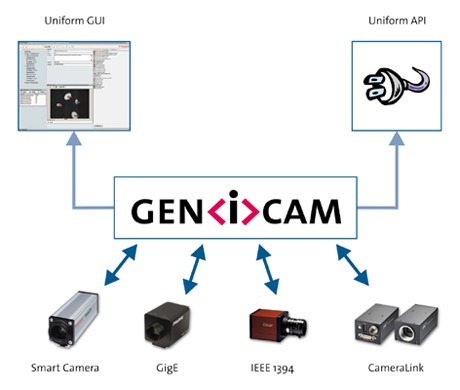
\includegraphics[width=0.8\textwidth]{images/genicam_protocol.jpg}
      \caption{Koncept GenICam protokolu \cite{genicamProtocolImage}}
      \label{fig:genicam_protocol}
	\end{figure}      
    
    \subsection{Dostupný software}
       Existují již hotové programy pro práci se stacionárními termokamerami, ale i~v ~placených verzích těchto softwarů nelze nalézt všechna potřebné nastavení a funkce. Je to z~toho důvodu, že tyto softwary jsou většinou pro průmyslové aplikace jako je monitoring, tvorbu reportů a ostatní komerční činnosti. 
       
       Příkladem je placený software FLIR Tools+ \cite{flirtools} přímo od výrobců termokamer FLIR. Tento software podporuje přenos obrazu z~kamery a jeho následné zobrazení, ale snímky jsou přenášeny pouze v~8-bitovém formátu. Dále nedovoluje ukládání surových dat, nepodporuje kontinuální ukládání a~ani zásah do nastavení kamery. 
       
       Všechny nalezené alternativní softwary mají též velmi omezené možnosti a~funkce. Kvůli tomu je vhodné využít SDK a zabývat se tvorbou vlastní aplikace pro ovládání kamery a získání snímku pro nutné potřeby řešení této práce. 
    
    \subsection{Sada vývojových nástrojů}\label{section:sdk}
    Lepším řešením, ale bohužel časově náročnějším, je využít vhodnou sadu vývojových nástrojů (SDK) a s~kamerou pracovat na úrovni kódu. Kamera FLIR A65 podporuje rozhraní GigE a GenICam a ač byly oba standardy vytvořeny již v~roce 2006, dostupných SDK je v~řádu jednotek. Nejčastěji využívané jsou:
      
    \begin{itemize}[noitemsep]
    \item Atlas SDK \cite{atlasSdk},
    \item JAI SDK \cite{jaiSdk},
    \item ActiveGigE \cite{activeGige},
    \item eBUS SDK \cite{ebusSdk}.
    \end{itemize}
      
    Všechny výše uvedené SDK podporují standardy GigE Vision a GenICam. Liší se použitým programovacím jazykem, kvalitou dokumentace, množstvím ukázkových programů a také dostupností. Stručně shrnuto:
    
    \begin{description}[align=left]
	\item [Atlas SDK] je dostupné pouze k~zakoupeným kamerám značky FLIR. Práce s~Atlas SDK probíhá v~jazyce C\# nebo prostředí MATLABu. Práce s~Atlas SDK je velmi snadná, má velmi dobrou dokumentaci a ukázkové kódy. Jedinou nevýhodou je omezený přístup k~nastavování jednotlivých parametrů protokolu.
    \item [JAI SDK] je produkt od výrobců průmyslových kamer JAI. V~současné době se firma JAI podílí také na rozvíjení standardů GigE Vision a GenICam. Jejich SDK je možné využívat v~jazyce C/C++ nebo v~C\#. Je zdarma, obsahuje velmi detailní dokumentaci a dostatečné množství ukázkových kódů. Součástí SDK je ovladač Filter driver pro urychlení přenosu dat. 
    \item [ActiveGigE] je SDK firmy A\&B Software. Na rozdíl od jiných SDK ho lze využít ve spoustě různých prostředích a programovacích jazycích. Je dostupné pro: Visual Studio, Visual Basic (VB), Delphi, PowerBuilder, Java, Matlab, Python, QT, Adobe Flash, LabView, GE Fanuc, Indusoft Studio. Zajímavou záležitostí je vkládání ActiveGigE objektů přímo do programů od Microsoftu (Word, PowerPoint) s~možností přenosu reálného obrazu. Ze všech porovnávaných SDK obsahuje v~základu nejvíce implementovaných funkcí. Samozřejmostí je rozsáhlá dokumentace a~ukázkové kódy. Jedinou nevýhodou se zdá být cena, ta je k~dubnu 2017 stanovena na 495 dolarů za licenci.
    \item [eBUS SDK] je od firmy Pleora, která se stejně jako JAI podílí na rozvíjení standardů pro strojové vidění. Je dostupné jak pro jazyk C/C++, tak pro C\#. Jeho použití je díky rozsáhlé dokumentaci a ukázkovým zdrojovým kódům velmi snadné. Součástí eBUS SDK je také ovladač Universal Pro Driver pro zvýšení propustnosti síťového rozhraní a snížení zátěže. eBUS SDK je pro kamery FLIR dostupné zdarma, pro kamery ostatních výrobců je licence zpoplatněna.
    \end{description}
    


